%
% This is a borrowed LaTeX template file for lecture notes for CS267,
% Applications of Parallel Computing, UCBerkeley EECS Department.
% Now being used for CMU's 10725 Fall 2012 Optimization course
% taught by Geoff Gordon and Ryan Tibshirani.  When preparing 
% LaTeX notes for this class, please use this template.
%
% To familiarize yourself with this template, the body contains
% some examples of its use.  Look them over.  Then you can
% run LaTeX on this file.  After you have LaTeXed this file then
% you can look over the result either by printing it out with
% dvips or using xdvi. "pdflatex template.tex" should also work.
%

\documentclass[twoside]{article}
\setlength{\oddsidemargin}{0.25 in}
\setlength{\evensidemargin}{-0.25 in}
\setlength{\topmargin}{-0.6 in}
\setlength{\textwidth}{6.5 in}
\setlength{\textheight}{8.5 in}
\setlength{\headsep}{0.75 in}
\setlength{\parindent}{0 in}
\setlength{\parskip}{0.1 in}

%
% ADD PACKAGES here:
%

\usepackage{amsmath,amsfonts,graphicx,amsthm}

%
% The following commands set up the lecnum (lecture number)
% counter and make various numbering schemes work relative
% to the lecture number.
%
\newcounter{lecnum}
\renewcommand{\thepage}{\thelecnum-\arabic{page}}
\renewcommand{\thesection}{\thelecnum.\arabic{section}}
\renewcommand{\theequation}{\thelecnum.\arabic{equation}}
\renewcommand{\thefigure}{\thelecnum.\arabic{figure}}
\renewcommand{\thetable}{\thelecnum.\arabic{table}}

%
% The following macro is used to generate the header.
%
\newcommand{\lecture}[4]{
   \pagestyle{myheadings}
   \thispagestyle{plain}
   \newpage
   \setcounter{lecnum}{#1}
   \setcounter{page}{1}
   \noindent
   \begin{center}
   \framebox{
      \vbox{\vspace{2mm}
    \hbox to 6.28in { {\bf EE302 - Feedback Systems
	\hfill Spring 2019} }
       \vspace{4mm}
       \hbox to 6.28in { {\Large \hfill Lecture #1 \hfill} }
       \vspace{2mm}
       \hbox to 6.28in { {\it Lecturer: #2 \hfill } }
      \vspace{2mm}}
   }
   \end{center}
   \markboth{Lecture #1}{Lecture #1}

   \vspace*{4mm}
}
%
% Convention for citations is authors' initials followed by the year.
% For example, to cite a paper by Leighton and Maggs you would type
% \cite{LM89}, and to cite a paper by Strassen you would type \cite{S69}.
% (To avoid bibliography problems, for now we redefine the \cite command.)
% Also commands that create a suitable format for the reference list.
\renewcommand{\cite}[1]{[#1]}
\def\beginrefs{\begin{list}%
        {[\arabic{equation}]}{\usecounter{equation}
         \setlength{\leftmargin}{2.0truecm}\setlength{\labelsep}{0.4truecm}%
         \setlength{\labelwidth}{1.6truecm}}}
\def\endrefs{\end{list}}
\def\bibentry#1{\item[\hbox{[#1]}]}

%Use this command for a figure; it puts a figure in wherever you want it.
%usage: \fig{NUMBER}{SPACE-IN-INCHES}{CAPTION}
\newcommand{\fig}[3]{
			\vspace{#2}
			\begin{center}
			Figure \thelecnum.#1:~#3
			\end{center}
	}
% Use these for theorems, lemmas, proofs, etc.
\newtheorem{theorem}{Theorem}[lecnum]
\newtheorem{lemma}[theorem]{Lemma}
\newtheorem{proposition}[theorem]{Proposition}
\newtheorem{claim}[theorem]{Claim}
\newtheorem{corollary}[theorem]{Corollary}
\newtheorem{definition}[theorem]{Definition}

\theoremstyle{definition}
\newtheorem{exmp}[theorem]{Ex}

%\newenvironment{proof}{{\bf Proof:}}{\hfill\rule{2mm}{2mm}}


% **** IF YOU WANT TO DEFINE ADDITIONAL MACROS FOR YOURSELF, PUT THEM HERE:

\begin{document}

% Lecture Details
\lecture{3}{Asst. Prof. M. Mert Ankarali}

\par 

\section{Modeling of Mechanical Systems and Their Electrical Analogy}

We use Kirchhoff's Current and Voltage laws to derive the 
dynamical (and static) relationships in Electrical Circuits. Similarly,
we utilize Newton's laws of motion to derive equations of motion
in (rigid body) mechanical dynamical systems. 

\subsection{Mechanical vs. Electrical Analogy Between Dependent Variables}

There exist two different analogies that we can construct between electrical and
mechanical systems. Mathematically, there is no difference between the two approaches. In 
this lecture, we will learn one of these analogies. 

In electrical circuits, the core variables are Voltage, $V$, and current, $I$, whereas
in translational mechanical systems, core variables are translational velocity, $\nu$, and force, $f$.
Similarly, in rotational mechanical systems, the core variables are angular velocity, $\omega$n, and torque $\tau$.

\textbf{Voltage, $V$ $\Longleftrightarrow$ Velocity, $\nu$
  $\Longleftrightarrow$ Angular Velocity, $\omega$}

In electrical systems, voltage, also called electric potential difference, accounts for the difference in electric potential between two points. When we refer to the voltage of a node/point, we  always measure it with respect to a reference point, e.g. \textit{ground}. In mechanical systems, we measure the velocity either between two points in space, or (which is more general) with respect to an inertial reference frame, e.g. \textit{ground} or \textit{earth} in general. The analogy is similar with angular velocity. For this reason, we say that voltage, linear velocity, and angular velocity are the analog variables.

\textbf{Current, $I$ $\Longleftrightarrow$ force, $f$
  $\Longleftrightarrow$Torque, $\tau$}

In electrical systems, the current is the flow (or rate of change of) of
electric charge and carried by electrons in motion. Roughly speaking, 
based on Newton's second law, the force acting upon a (rigid) body is equal to the rate of change of momentum related to this specific
force component. Momentum can be considered as an analog of the
electrical charge in this case. A similar analogy can also be
constructed using Torque and Angular Momentum. For this reason, we say that Current, Force, and Torque are the analog variables.

\subsection{Capacitor $C$, 1-DOF Translating Body with Mass
  $m$, and 1-DOF Rotating Body with Inertia $J$}

If we follow the analogs between the variables, we can see that ideal
capacitor for which one end is connected to the ground, 1-DOF translating body with a mass
of $m$, and 1-DOF rotating body with an inertia of  $J$ analogs of each other. 
These are all ideal energy storage elements in their modeling
domains and they are illustrated in the figure below. 

  \begin{minipage}[h]{0.95\linewidth}
    \begin{center}
      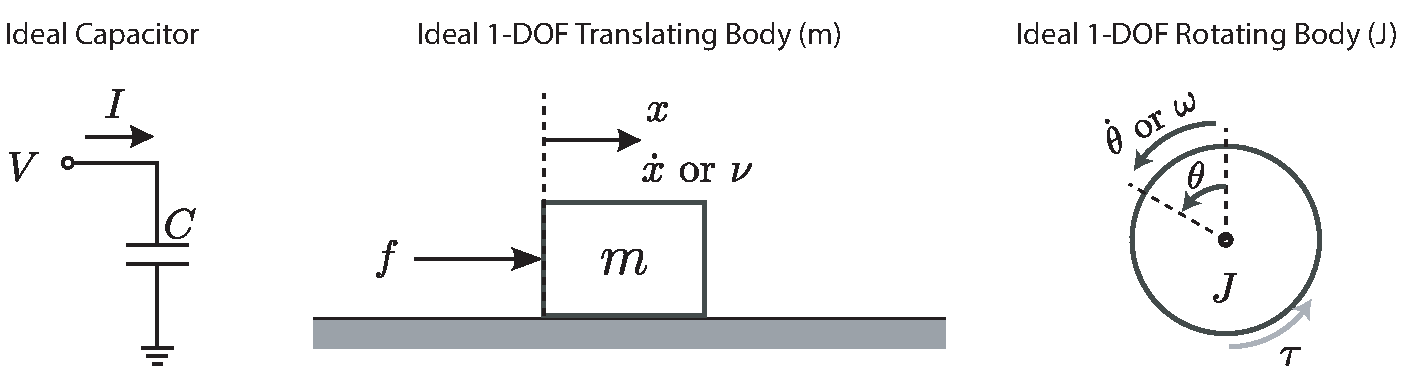
\includegraphics[width=1\textwidth]{cap}
    \end{center}
  \end{minipage}

The ODEs that govern the dynamics of these elements are provided below
%
\begin{align*}
\mathrm{Capacitor:}& \quad C \dot{V}(t) = I(t) \\
\mathrm{Mass:}& \quad  m \dot{\nu} = f(t) \ (\mathrm{or} \ m \ddot{x} =
                f(t) ) \\
\mathrm{Inertia:}& \quad J \dot{\omega} = \tau (t) \ (\mathrm{or} \ J \ddot{\theta} = \tau (t) )
\end{align*}
%
Based on these equations we can reach the following (system) parameter
analogy as
%
\begin{align*}
 C \equiv m \equiv J
\end{align*}
%

\subsection{Inductor $L$, Translational Spring $k$, and Torsional Spring $\kappa$}

If we follow the analogs between the variables we can see that Ideal
inductor ($L$), linear translational spring ($k$), and linear
torsional spring ($\kappa$) are analogs of each other. 
These are also ideal energy storage elements in their modeling
domains and they are illustrated in the figure below. 

  \begin{minipage}[h]{1\linewidth}
    \begin{center}
      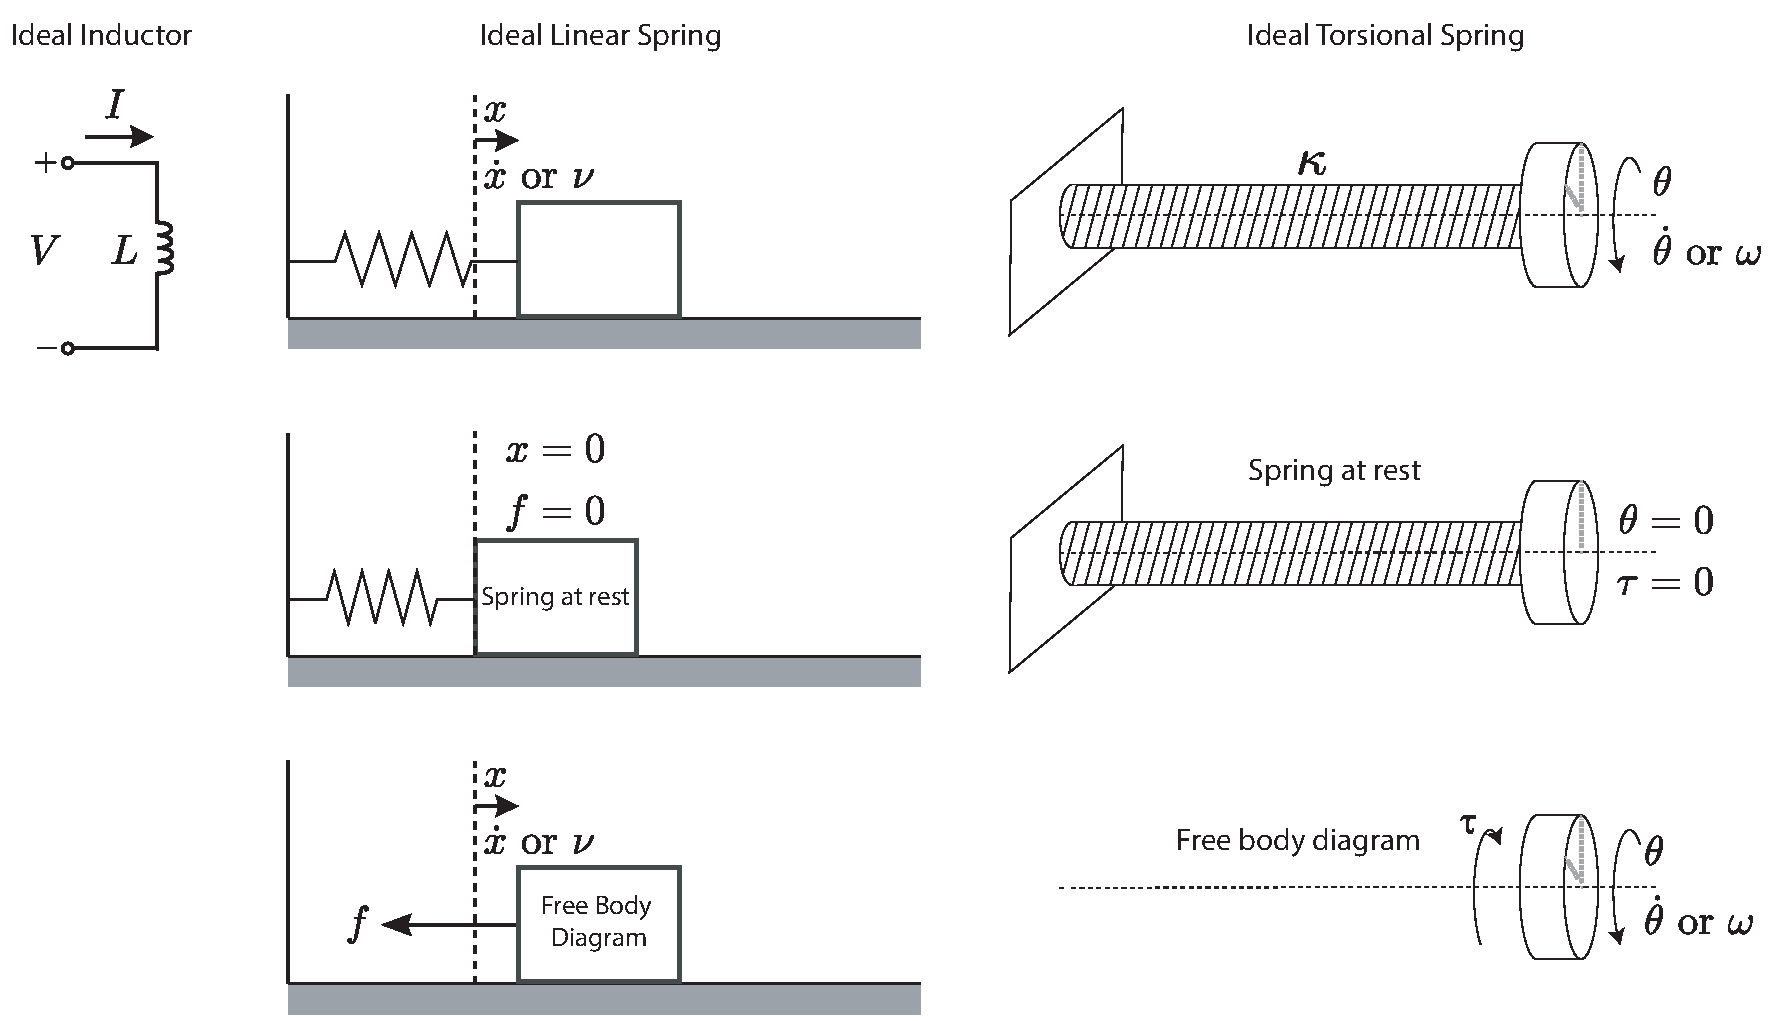
\includegraphics[width=1\textwidth]{ind}
    \end{center}
  \end{minipage}

The ODEs that govern the dynamics of these elements are provided below
%
\begin{align*}
\mathrm{Induction:}& \quad L \dot{I}(t) = V(t) \\
\mathrm{Translational Spring:}& \quad  f(t) = k x(t) \ \rightarrow \
                                \frac{1}{k} \dot{f}(t) = \nu(t)
\\
\mathrm{Torsional Spring:}& \quad  \tau (t) = \kappa \theta(t) \
                            \rightarrow \ \frac{1}{\kappa} \dot{\tau}(t) = \omega(t)
\end{align*}
%
Based on these equations we can reach the following (system) parameter
analogy as
%
\begin{align*}
 L \equiv \frac{1}{k} \equiv \frac{1}{\kappa}
\end{align*}
% 

\subsection{Resistor $R$, Damper (Viscous Friction) $b$, and
Torsional Damper $\beta$}

If we follow the analogs between the variables we can see that Ideal
resistor ($R$), linear translational damper ($k$), and linear
torsional damper ($\kappa$) are analogs of each other. 
These elements are ideal fully passive dissipative elements.
Thus, these are memoryless (static) components as opposed to the
previous elements. These elements are illustrated in the figure below. 

  \begin{minipage}[h]{1\linewidth}
    \begin{center}
      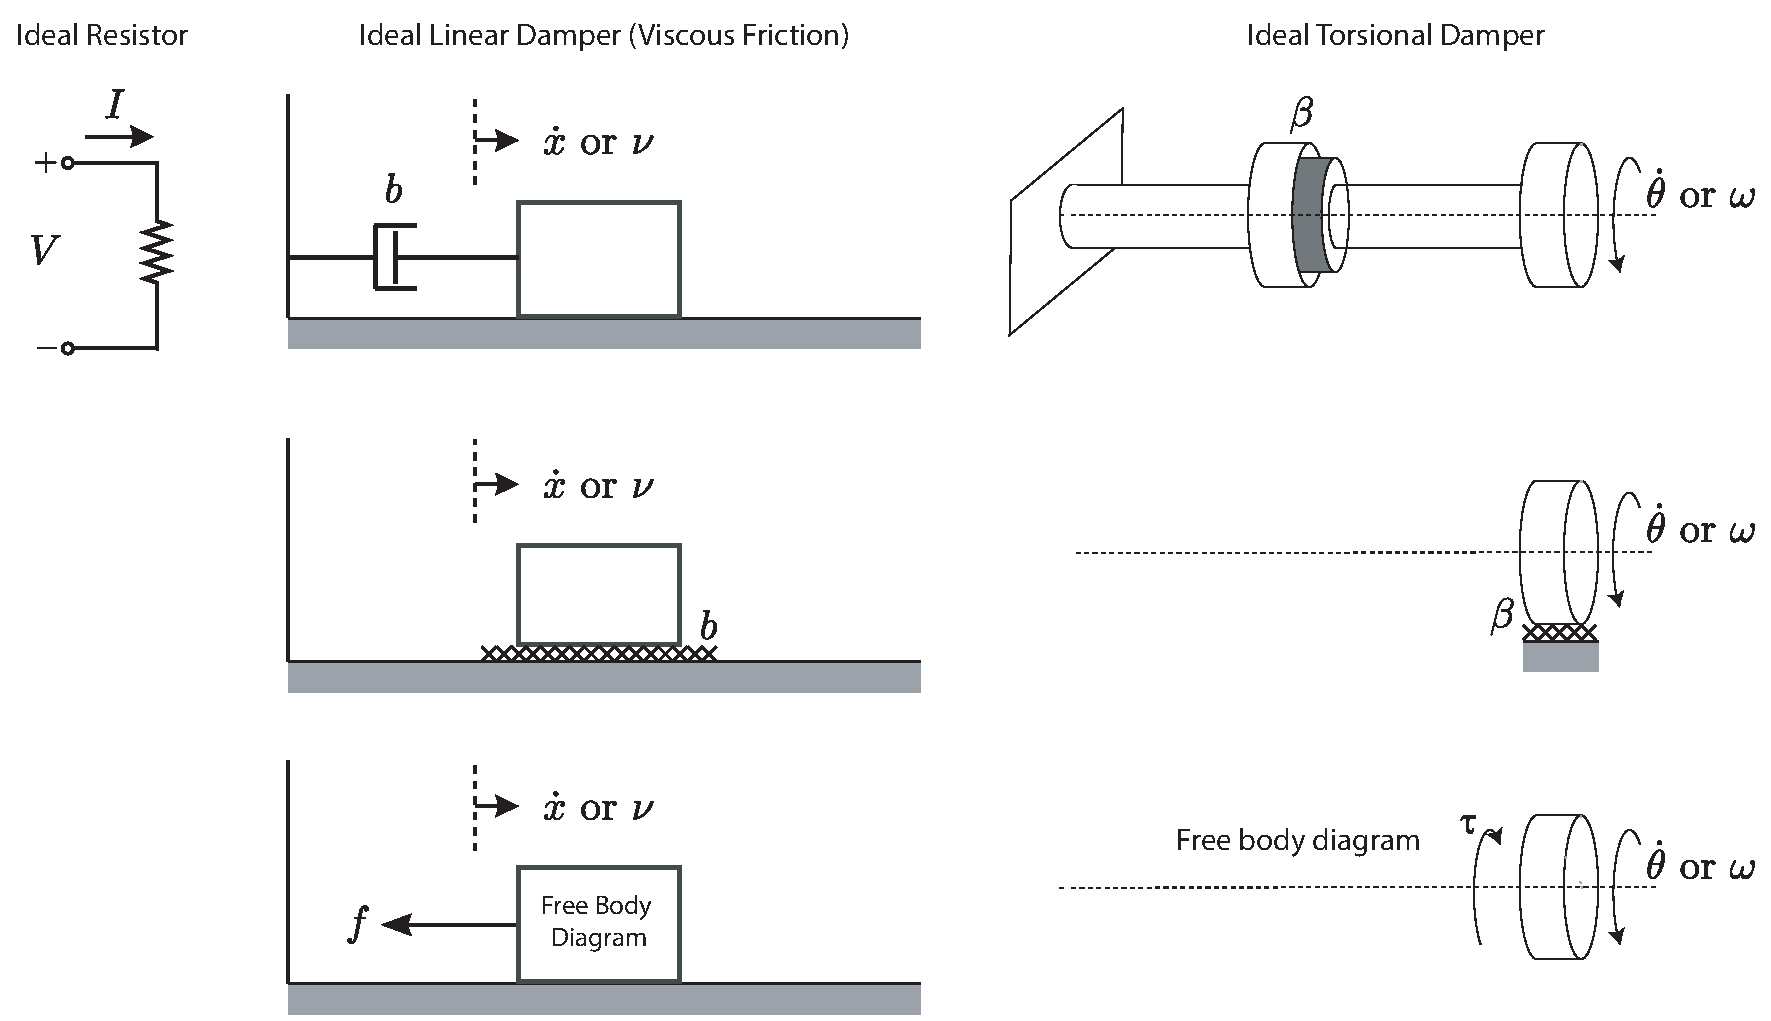
\includegraphics[width=1\textwidth]{res}
    \end{center}
  \end{minipage}

The algebraic equations that govern the statics of these elements are provided below
%
\begin{align*}
\mathrm{Resistor:}& \quad V(t) = R I(t)   \\
\mathrm{Translational} \ \mathrm{Damper:}& \quad  f(t) = b \dot{x}(t) \ \mathrm{or} \
                                \frac{1}{b} f(t) = \nu(t) 
\\
\mathrm{Torsional} \ \mathrm{Damper:}& \quad  \tau (t) = \beta \dot{\theta}(t) \
                            \rightarrow \ \frac{1}{\beta} \tau(t) = \omega(t)
\end{align*}
%
Based on these equations we can reach the following (system) parameter
analogy as
%
\begin{align*}
 R \equiv \frac{1}{b} \equiv \frac{1}{\beta}
\end{align*}
% 



\subsection{Ideal Transformer, Linearized Lever, and
Gear Pair}

In both electrical and mechanical systems, we have transmission
elements. In their ideal form, they conserve the energy after the transformation. In electrical
systems, transformer is the component that achieves the transmission.
In translational mechanical systems a linearized lever can achieve this
under the assumption of small movements, where as for rotational
systems a gear pair is one of the many solutions for mechanical
transmission. These components are illustrated in the figure below. 

  \begin{minipage}[h]{1\linewidth}
    \begin{center}
      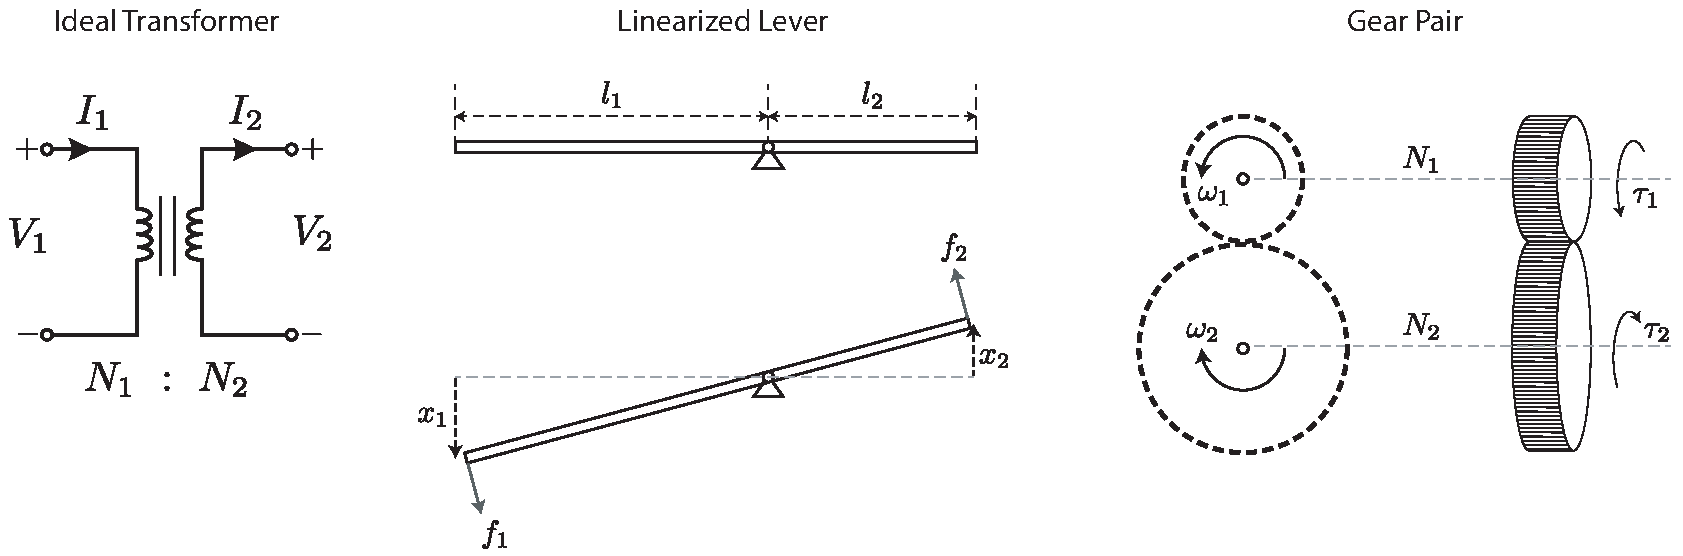
\includegraphics[width=1\textwidth]{trans}
    \end{center}
  \end{minipage}

The algebraic equations that govern the statics of these elements are provided below
%
%
\begin{align*}
\mathrm{Electrical} \ \mathrm{Transformer:}& \begin{array}{c} \frac{V_1}{N_1} =
                                    \frac{V_2}{N_2} \\ \\ I_1 N_1 = I_2 N_2 \end{array} 
\\ \\
\mathrm{Lever:}& \quad  \begin{array}{c} \frac{\nu_1}{l_1} =
                                    \frac{\nu_2}{l_2} \\ \\ f_1 l_1 = f_2 l_2 \end{array} 
\\ \\
\mathrm{Gear-Pair:}& \quad  \begin{array}{c} \frac{\omega_1}{r_2} =
                                    \frac{\omega_2}{r_1} \\ \\ \tau_1 r_2 = \tau_2 r_1 \end{array} 
\end{align*}
%
Based on these equations, it is to see that following (system) parameter
analogy as
%
\begin{align*}
\frac{N_1}{N_2} \equiv \frac{l_1}{l_2} \equiv \frac{r_2}{r_1} 
\end{align*}
%

\newpage

\section{Examples}

\begin{exmp}
Let's consider the following translational mechanical system. The
input of the system is $v_i(t)$ which is the velocity of the one side
of the first damper. The output of the system is $v_m(t)$, i.e. the velocity of the mass. 
\end{exmp}

  \begin{minipage}[h]{0.5\linewidth}
    \begin{center}
      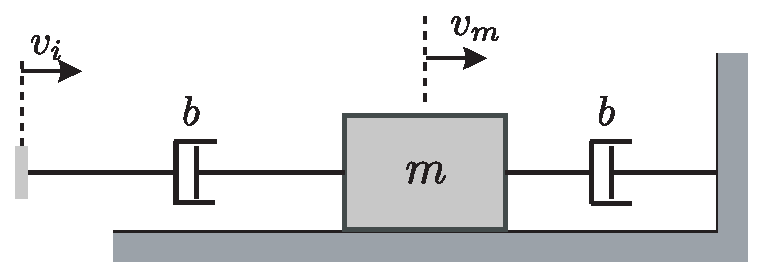
\includegraphics[width=1\textwidth]{example}
    \end{center}
  \end{minipage}

  \vspace{6pt}

\begin{enumerate}

\item Given that $u(t) = v_i(t)$ and $y(t) = v_m(t)$, find the transfer
function $G(s) = \frac{Y(s)}{U(s)}$

\vspace{6pt}

Let's first draw the FBD and then derive the equations
of motion

  \begin{minipage}[h]{0.5\linewidth}
    \begin{center}
      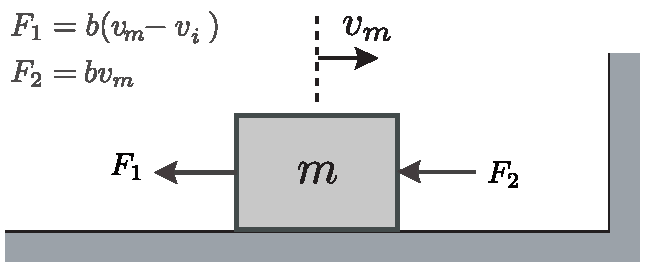
\includegraphics[width=1\textwidth]{example_sol}
    \end{center}
  \end{minipage}
  \begin{minipage}[h]{0.5\linewidth}
    \begin{center}
 	\begin{align*}
	&m \dot{v}_m = -F_1 - F_2 = b v_i - 2 b v_m 
	\\
        &m \dot{y}  + 2 b y = b u
         \\
         &G(s) =  \frac{Y(s)}{U(s)} = \frac{b}{m s + 2 b} =
           \frac{b/m}{s + (2 b)/m} 
		\end{align*}
    \end{center}
   \end{minipage}

\item Now, let's construct an electrical circuit analog of the mechanical system.

Let 
%
\begin{align*}
	V_i \equiv v_i
	\quad 
	I_i \equiv f_i
\end{align*}
%
then we can build the circuit analog as in the illustration below. 

  \begin{minipage}[h]{0.4\linewidth}
    \begin{center}
      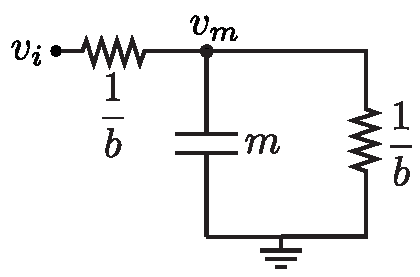
\includegraphics[width=1\textwidth]{example_elec}
    \end{center}
  \end{minipage}

\item Finally, compute $G(s)$ by analyzing the
  electrical analog circuit.

We simply apply KCL

\begin{align*}
  \frac{v_i - v_m}{1/b} &= I_m + \frac{v_m}{1/b} \quad \Rightarrow
                          \quad I_m = m \dot{v}_m
\\
    b v_i &= m \dot{v}_m + 2 b v_m \quad \Rightarrow
                          \quad     b u = m \dot{y} + 2 b y
\\
G(s) &= \frac{Y(s)}{U(s)} = \frac{b/m}{s + (2b)/m}
\end{align*}

\end{enumerate}

\vspace{6pt}

\begin{exmp} Let's consider the following translational mechanical system. It is given that when the lever is in vertical position, 
$\left[ x_0 \ x_1 \ x_2 \right] = 0$ and springs are at their rest length positions. 
\end{exmp}

\begin{enumerate}

\item Given that $u(t) = x_0(t)$ and $y(t) = x_2(t)$,
find the ODE of the system dynamics.
 
\vspace{6pt}

  \begin{minipage}[h]{0.6\linewidth}
    \begin{center}
      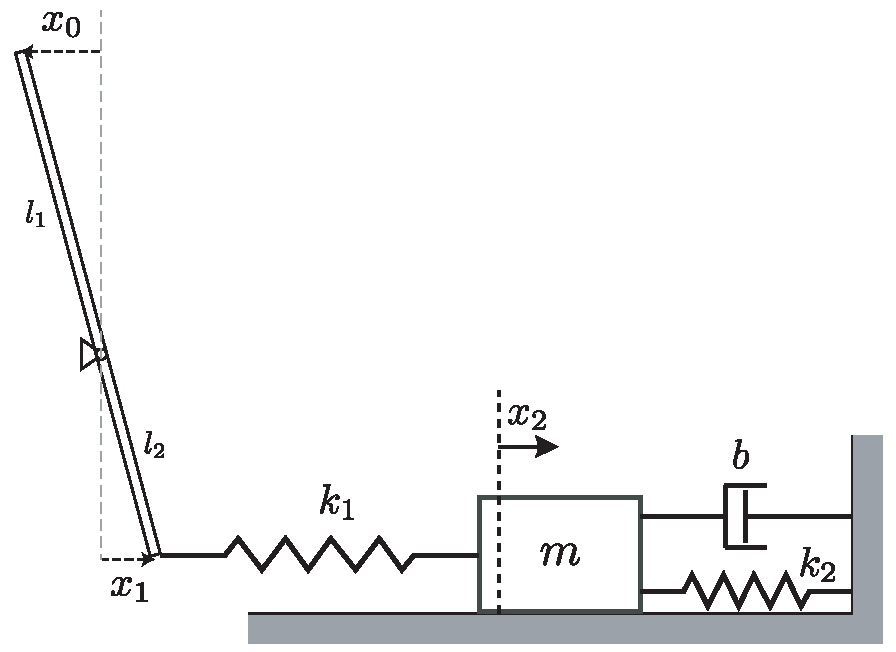
\includegraphics[width=1\textwidth]{ex1}
    \end{center}
  \end{minipage}
  \begin{minipage}[h]{0.4\linewidth}
    \begin{center}
 	\begin{align*}
	&m \ddot{x_2} = - b \dot{x}_2 - k_2 x_2 + k_1 (x_1 - x_2)
	\\
	&x_1  = x_0 \frac{l_2}{l_1} 
	\\
	&m \ddot{x_2} + b \dot{x}_2 + (k_1 + k_2) x_2  =  k_1 \frac{l_2}{l_1} x_0
	\\
	&\ddot{y} + \frac{b}{m} \dot{y} + \frac{k_1 + k_2}{m} y  = 
	\frac{k_1}{m} \frac{l_2}{l_1} u
		\end{align*}
    \end{center}
  \end{minipage}
  
  \vspace{6pt}
  
  \item Find the transfer function for same input-output pair.
{\large  
\begin{align*}
G(s) = \frac{Y(s)}{U(s)} = \frac{\frac{k_1}{m} \frac{l_2}{l_1}}{s^2 + \frac{b}{m} s + \frac{k_1 + k_2}{m}}  
\end{align*}
}

\item Now, let's construct an electrical circuit analog of the mechanical system.

Let 
%
\begin{align*}
	V_i \equiv \dot{x}_i
	\\
	I_i \equiv f_i
\end{align*}
%
then we can build the circuit analog as in the illustration below. 

  \begin{minipage}[h]{0.75\linewidth}
    \begin{center}
      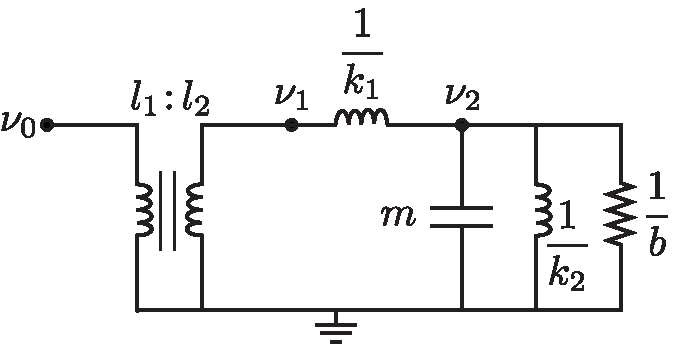
\includegraphics[width=1\textwidth]{ex_elec}
    \end{center}
  \end{minipage}
  
  Let's also compute 
$\frac{\mathcal{V}_2(s)}{\mathcal{V_0}(s)}$ using node voltage analysis in impedance domain.

\begin{align*}
	\frac{\mathcal{V}_2(s) - \mathcal{V}_1(s) }{ \frac{s}{k_1} } + 
	\frac{\mathcal{V}_2(s)}{ \frac{1}{m s} } + 	\frac{\mathcal{V}_2(s)}{ \frac{s}{k_2} } +
	\frac{\mathcal{V}_2(s)}{ \frac{1}{b} } 
	= 0 
	\\
	\mathcal{V}_2(s) \left[ m s + b + \frac{k_1+k_2}{s} \right] = V_1(s) \left[  \frac{k_1}{s} \right]
	\\
	\mathcal{V}_2(s) \left[ m s^2 + b s + ( k_1 + k_2) \right] = V_1(s) \left[  k_1 \right]
\end{align*}

Since ideal transformer has the following relation, $\mathcal{V}_1(s) = \frac{l_2}{l_1} \mathcal{V}_0(s)$, 
we have the following transfer function between $\mathcal{V}_0(s)$ and $\mathcal{V}_2(s)$

\begin{align*}
\frac{\mathcal{V}_2(s)}{\mathcal{V}_0(s)} = \frac{\frac{k_1}{m} \frac{l_2}{l_1}}{s^2 + \frac{b}{m} s + \frac{k_1 + k_2}{m}}  
\end{align*}

Obviously this transfer function is equal to $G(s)$ computed from directly mechanical system and considering positional variables.

\item Convert the derived ODE into a state-space form
%

We will solve the problem using a different approach. First let's
integrate the ODE twice

\begin{align*}
  y =  \int \left[ - \frac{b}{m} y + \int \left\lbrace - \frac{k_1 + k_2}{m} y  +
	\frac{k_1}{m} \frac{l_2}{l_1} u \right\rbrace dt \right] dt
\end{align*}

Then let the stat variable definitions be
%
\begin{align*}
  x_1 &= y = \int \left[ - \frac{b}{m} y + \int \left\lbrace - \frac{k_1 + k_2}{m} y  +
	\frac{k_1}{m} \frac{l_2}{l_1} u \right\rbrace dt \right] dt \\
  x_2 &= \int \left\lbrace - \frac{k_1 + k_2}{m} y  +
	\frac{k_1}{m} \frac{l_2}{l_1} u \right\rbrace dt
\end{align*}
%
Then state-equations take the form
%
\begin{align*}
  \dot{x}_1 &= \left[ - \frac{b}{m} y + \int \left\lbrace - \frac{k_1 + k_2}{m} y  +
	\frac{k_1}{m} \frac{l_2}{l_1} u \right\rbrace dt \right] \\
  &= - \frac{b}{m} x_1 + x_2 \\
  \dot{x}_2 &= \left\lbrace - \frac{k_1 + k_2}{m} y  +
	\frac{k_1}{m} \frac{l_2}{l_1} u \right\rbrace
\\ 
&= - \frac{k_1 + k_2}{m} x_1  +
	\frac{k_1}{m} \frac{l_2}{l_1} u 
\end{align*}
%
If we gather the obtained state-equations in matrix form we obtain the
following state-space representation
%
\begin{align*}
  \dot{x} &= \left[ \begin{array}{cc} - \frac{b}{m} & 1 \\ - \frac{k_1
                     + k_2}{m} & 0 \end{array} \right] x +
  \left[ \begin{array}{c} 0 \\ \frac{k_1}{m}
           \frac{l_2}{l_1}  \end{array} \right] u 
\\
y &= \left[ \begin{array}{cc} 1 & 0 \end{array} \right] x
\end{align*}

\end{enumerate}

\vspace{12pt}

\begin{exmp} Let's consider the following gear system. Unlike ideal gear pair case, now each gear has its own inertia, $J_1$ and
$J_2$, as well as both gears are affected by viscous friction,
$\beta_1$ and $\beta_2$ , due to mechanical contact with the
environment. 
\end{exmp}

    \begin{center}
  \begin{minipage}[h]{0.75\linewidth}
    \begin{center}
      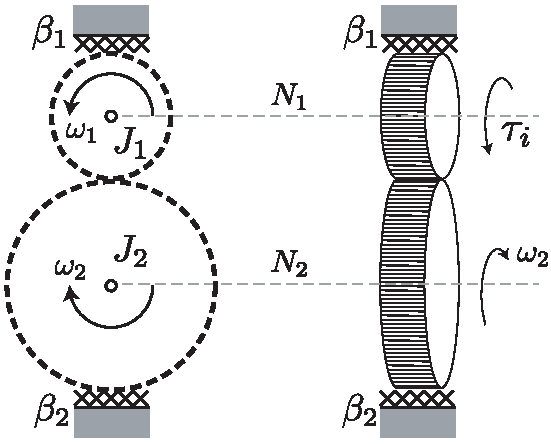
\includegraphics[width=1\textwidth]{ex2}
    \end{center}
  \end{minipage}
    \end{center}

\begin{enumerate}

\item Given that there is an external torque, $\tau_i$, acting on the first gear is the input of the system, and the rotational speed of the
second gear, $\omega_2$, is the output of the system, find the ODE of the gear-box dynamics. 

First let's draw the free-body diagrams of both gears separately and then write the equations of motion for each body. 


  \begin{minipage}[h]{0.35\linewidth}
    \begin{center}
      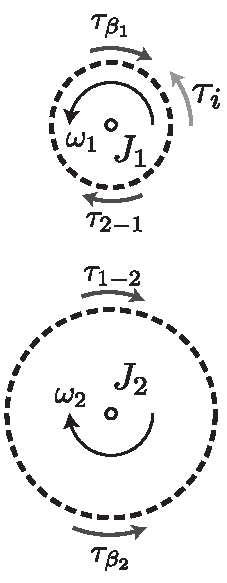
\includegraphics[width=0.95\textwidth]{ex2_sol}
    \end{center}
  \end{minipage}
\begin{minipage}[h]{0.65\linewidth}

 	\begin{align*}
	J_1 \dot{\omega_1} &= \tau_i - \tau_{\beta_1} - \tau_{2-1}
	\\
	&= \tau_i - \beta_1 \omega_1 - \tau_{2-1}
	\\
	J_2 \dot{\omega_2} &= -\tau_{\beta_2} + \tau_{1-2}
			\\
		&= -\beta_2 \omega_2 + \tau_{1-2}
	\end{align*}
    %
    Based on the gear kinematics we know that 
    %
    \begin{align*}
    	\omega_1 &= \frac{N_2}{N_1} \omega_2
	\\
	\tau_{1-2}  &= \frac{N_2}{N_1}  \tau_{2-1} 
    \end{align*}
    %
    Thus we have the following derivations
    %
     	\begin{align*}
	\tau_{2-1} &=  \tau_i  - J_1  \frac{N_2}{N_1} \dot{\omega_2} - \beta_1 \frac{N_2}{N_1} \omega_2 
	\\
	\tau_{1-2} &=   \frac{N_2}{N_1}  \tau_i  - J_1  \left(\frac{N_2}{N_1}\right)^2 \dot{\omega_2} - \beta_1 \left(\frac{N_2}{N_1}\right)^2 \omega_2 
	\end{align*}
	%
	Hence the ODE governing the dynamics can be formed as
	%
	\begin{align*}
	\left[ J_2 + J_1  \left(\frac{N_2}{N_1}\right)^2  \right] \dot{y}
	+ \left[ \beta_2 + \beta_1 \left(\frac{N_2}{N_1}\right)^2  \right]  y
	= \frac{N_2}{N_1}  u
	\end{align*}
    
  \end{minipage}

It can be seen that the resultant ODE is a first order ODE. Ee can also consider the whole system as a
single rotating body with an effective total inertia of $J_T = \left[ J_2 + J_1  \left(\frac{N_2}{N_1}\right)^2  \right]$
and effective total viscous friction of $\beta_T  = \left[ \beta_2 + \beta_1 \left(\frac{N_2}{N_1}\right)^2 \right]$.  

\vspace{12pt}
  
 \textbf{Take Home Problem:} Now let's assume that output is $y(t) = \omega_1(t)$, and govern the ODE and re-compute
 the new effective inertia and viscous friction.  

\item Compute the transfer function

\begin{align*}
	G(s) &= \frac{Y(s)}{U(s)} = 
	\frac{ \frac{N_2}{N_1}  }{ \left[ J_2 + J_1  \left(\frac{N_2}{N_1}\right)^2  \right] s +  \left[ \beta_2 + \beta_1 \left(\frac{N_2}{N_1}\right)^2 \right]}
	\\
	&= 
	\frac{ \frac{N_2}{N_1}  }{ J_T s + \beta_T } = \frac{ \frac{N_2}{N_1} \frac{1}{J_T}  }{ s + \frac{\beta_T}{J_T} } 
\end{align*}
  
  \item Now, build the electrical circuit analog of the gear-box system
  
  \par
  
  The circuit diagram is given below
  
    \begin{minipage}[h]{0.75\linewidth}
    \begin{center}
      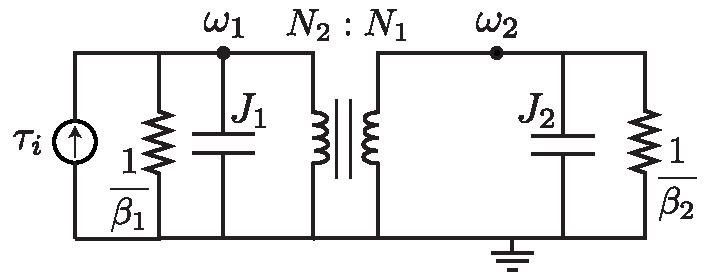
\includegraphics[width=1\textwidth]{ex2_elec}
    \end{center}
  \end{minipage}

\textbf{Take Home Problem:} Solve the electrical circuit and compute the transfer function $G(s)$   
  
\end{enumerate}

\vspace{12pt}

\begin{exmp} The figure below illustrates the model of the target system. Input of the system is the external torque, $u(t) = \tau(t)$, acting on the $R$ axis
and the output of the system is the angular velocity of the Load, i.e. $y(t) = \omega_L (t)$
\end{exmp}

\vspace{12pt}

\begin{minipage}[h]{1\linewidth}
    \begin{center}
      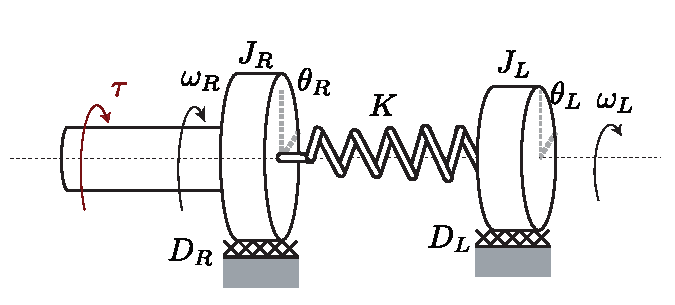
\includegraphics[width=0.99\textwidth]{system_model}
    \end{center}
\end{minipage}

Let's use the following state-definition 
%
\begin{align*}
  x(t) = \left[ \begin{array}{c} \omega_L \\ \omega_R \\ \theta_R - \theta_L \end{array} \right]
\end{align*}    
%
and then find a state-space representation for the system under this assumption. 
Indeed, since output is simply equal to one of the states, output equation is 
trivial 
%
\begin{align*}
  y(t) = \left[ \begin{array}{cccc} 1 & 0 & 0 \end{array} \right] x(t) + [0] u(t)
\end{align*}    
%  
Let's first write the differential equation on the motor axis
%
\begin{align*}
J_R \cdot \dot{\omega}_R &= \tau - D_R \omega_R  - \kappa (
                           \theta_R - \theta_L)
\end{align*}    
%  
If we replace the variables with state variables, we obtain. 
%
\begin{align*}
J_R \cdot \dot{x}_2 &= u - D_R x_2  - K x_3
\\
\dot{x}_2 &= \frac{1}{J_R} u - \frac{D_R}{J_R} x_2 - \frac{\kappa}{J_R} x_3
\end{align*}    
%  

Now let's write the differential equation on the load axis and perform
the same change of variables operation 
%
\begin{align*}
J_L \cdot \dot{\omega}_L &= \kappa ( \theta_R - \theta_L) - D_L \omega_L
\\
\dot{x}_1 &= \frac{K}{J_L} x_3 - \frac{D_L}{J_L} x_1
\end{align*}    
%
We need one more state-equation which can be drived as
%
\begin{align*}
   \dot{x}_3 = \frac{d}{dt} \left( \theta_R - \theta_L \right) =
  \omega_R - \omega_L = x_2 - x_1
\end{align*}
%
Based on our choice of state-definition, full state-space
representation takes the form
%
\begin{align*}
\dot{x}(t) &= \left[ \begin{array}{ccc} \frac{-D_L}{J_L} & 0 & \frac{\kappa}{J_L}  \\
0 & -\frac{D_R}{J_R} & -\frac{\kappa}{J_R} 
\\
-1 & 1 & 0 \\
\end{array} \right] x(t) +
                   \left[ \begin{array}{c} 0 \\ \frac{1}{J_R} \\
                            0 \end{array} \right] u(t)
\\
y(t) &= \left[ \begin{array}{ccc} 1 & 0 & 0 \end{array} \right] x(t) +
                                          [0] u(t)
\end{align*}    

%%%%%%%%%%%%%%%%%%%%%%%

\vspace{6pt}

\begin{exmp}
The mechanism illustration given below is an ideal belt-pulley
mechanism. Fundamentally, it has the same
kinematic relations with a gear pair system. The only difference is that, the direction of motion is preserved
in a pulley system. $r_1$ and $r_2$ correspond to the radii of the
first and second pulleys respectively. 
\end{exmp}
  
\vspace{12pt}
  
\begin{minipage}[h]{0.75\linewidth}
    \begin{center}
      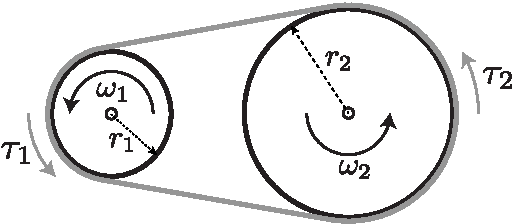
\includegraphics[width=0.8\textwidth]{beltpulley}
    \end{center}
\end{minipage}
\begin{minipage}[h]{0.25\linewidth}
    \begin{center}
\begin{align*}
	\frac{\omega_1}{r_2} &= \frac{\omega_2}{r_1}
	\\
	\frac{\tau_1}{r_1} &= \frac{\tau_2}{r_2}
\end{align*}
    \end{center}
\end{minipage}    

\vspace{12pt}

You will analyze the following belt-pulley system consisting of three pulleys and two belts. First pulley 
has a radius of $r_1$ and an inertia of $J_1$. Third pulley has a radius of $r_3$ and an inertia of $J_3$. 
Second pulley (in the middle) is connected to the first pulley through
its outer disk, which has the same radius with the third pulley, i.e.,
$r_{2,o} = r_3$. Second pulley is also connected to the first pulley
via its inner disk, which has the same radius with the first pulley, i.e.,
$r_{2,i} = r_1$. Second pulley has an inertia of $J_2$ (outer and
inner disks move together). A linear rotational viscous damping
with a damping constant $\beta_2$ also affects the motion of the
second pulley. 
	
\vspace{6pt} 
	
Given that the external torque acting on the first pulley is the input, $u(t) = \tau_{ex}(t)$, and the angular velocity of the third pulley
is the output, $y(t) = \omega_3(t)$, compute the transfer function of
the system.

\vspace{12pt}
	
	\begin{minipage}[h]{1\linewidth}
    \begin{center}
      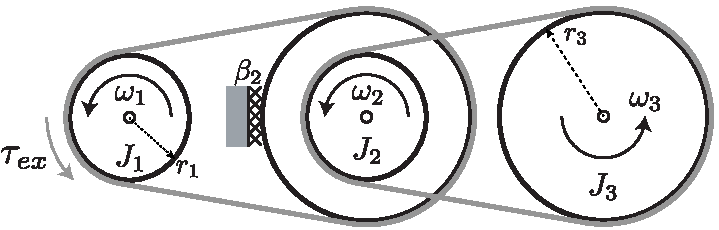
\includegraphics[width=0.9\textwidth]{beltpulleysystem}
    \end{center}
\end{minipage}

\vspace{12pt}

Let's solve this problem using the concept of reflected inertia, damping, and torque.
	
\vspace{6pt} 
	
If we reflect the variables and parameters of first pullet to the second pulley we obtain
	
\vspace{12pt}
	
	\begin{minipage}[h]{1\linewidth}
    \begin{center}
      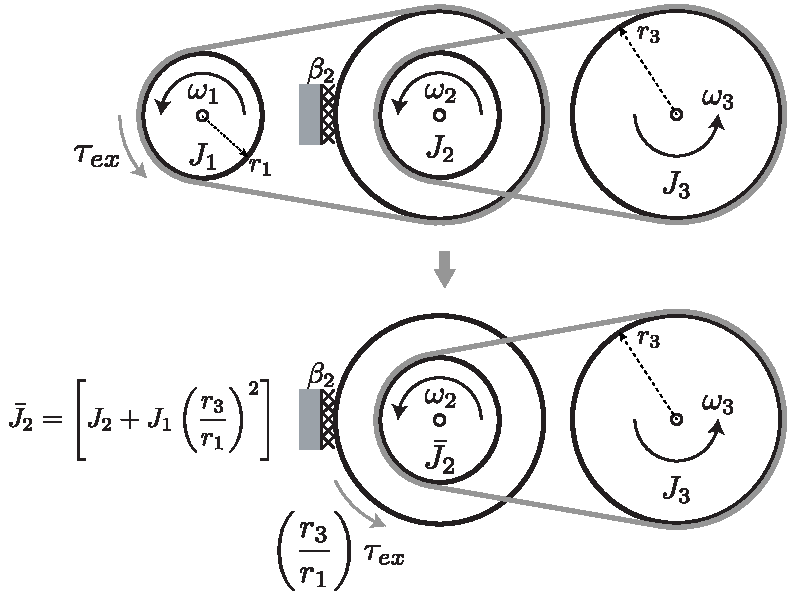
\includegraphics[width=0.9\textwidth]{beltpulleysystem_sol1}
    \end{center}
\end{minipage}
    
\vspace{12pt}

Now if we reflect the variables and parameters of the modified second pulley to the the third pulley we obtain
    
    \vspace{12pt}
	
	\begin{minipage}[h]{1\linewidth}
    \begin{center}
      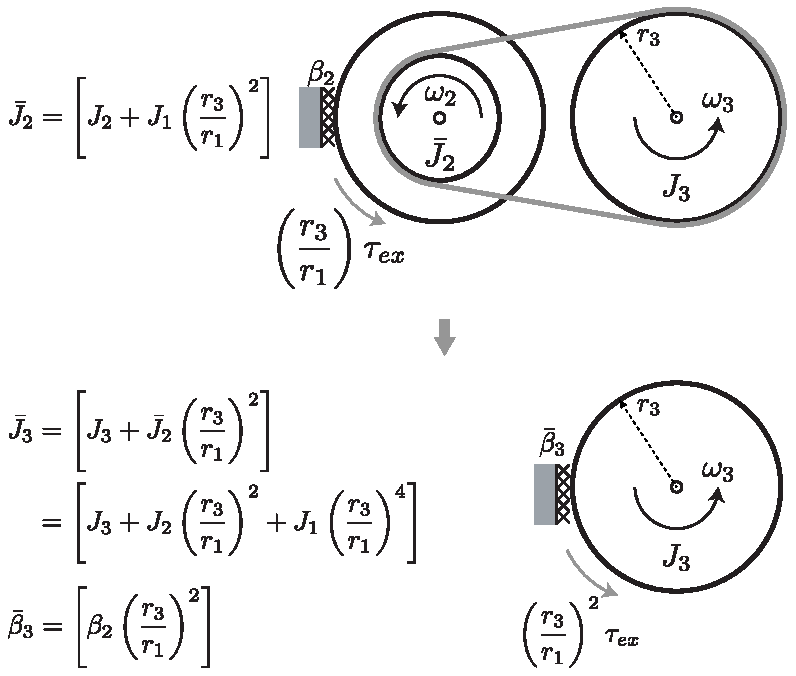
\includegraphics[width=0.9\textwidth]{beltpulleysystem_sol2}
    \end{center}
\end{minipage}
    
Hence, ode and transfer function of the system can be computed as
%
\begin{align*}    
\bar{J}_3 \dot{\omega_3} + \bar{\beta}_3 {\omega}_3 =
  \left( \frac{r_3}{r_1} \right)^2 \tau_{ex}
\quad &\rightarrow \quad 
\dot{y} + \frac{\bar{\beta}_3}{\bar{J}_3} = \frac{\left(
  \frac{r_3}{r_1} \right)^2}{\bar{J}_3} u
\\
\frac{Y(s)}{U(s)} &= \frac{\left(
  \frac{r_3}{r_1} \right)^2 \frac{1}{\bar{J_3}}}{s + \frac{\bar{\beta}_3}{\bar{J}_3}}
\end{align*}

%%%%%%%%%%%%%%%%%%%%%%%

\newpage

\begin{exmp}
In some belt-pulley applications, ignoring the
      elasticity of the belt can be very crude and can lead to 
      substantial modeling errors. 
    In order to overcome this problem, a very common method is modeling the belt with a linear (translational) spring-damper as shown in 
    the belt-pulley mechanism below. In this mechanism, first pulley
    has a radius of $r_1$ and inertia of $J_1$, where as the second pulley 
    has a radius of $r_2$ and inertia of $J_2$. The spring-mass dampers (above and below) that model the elasticity of the belt 
    have spring stiffnesses of $k$ and damping constants of $b$. 
\end{exmp}
    
    \vspace{12pt}
    
\begin{minipage}[h]{1\linewidth}
    \begin{center}
      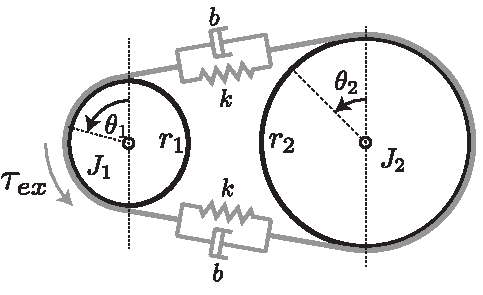
\includegraphics[width=0.9\textwidth]{beltpulleyelastic}
    \end{center}
\end{minipage}

\vspace{12pt}

Given that the external torque acting on the first pulley is the input, $u(t) = \tau_{ex}(t)$, and the angular displacement of the second pulley
is the output, $y(t) = \theta_2(t)$,

\begin{enumerate}
	\item Find a state-space representation of the dynamics. (\textit{Hint:} You can choose your state variables as $\mathbf{x} = \left[ \theta_1 \ \dot{\theta}_1 \
            \theta_2 \ \dot{\theta}_2 \right]^T$).
	\item Compute the transfer function, $G(s) = Y(s) / U(s)$
	\item Now, let the parameters of the system be equal to following numerical values
	\begin{align*}
		r_1 &= 0.05 \, m \  , \  r_2 = 0.1 \, m   \ , \  J_1 = 0.01 \, kg  \cdot m^2  
		 \ , \  J_2 = 0.1 \, kg  \cdot m^2  \\
		  k &= 100 \, N/m  \ , \ b = 10 \, N/(m \cdot s) \ .
	\end{align*}
	Simplify both the state-space and transfer function representations using these numerical values. 
	Finally convert the state-space form to the transfer function form and verify that converted transfer function
	is equal to the previously computed one. (\textit{Hint:} You can use MATLAB's \textit{ss2tf} command for conversion).
\end{enumerate}

We assume that when $[ \theta_1 \ \theta_2 \ \dot{\theta}_1
      \ \dot{\theta}_2 ] = [0 \ 0 \ 0 \ 0]$ the mechanism is at rest
      condition. Then let's draw the free-body diagrams
    
    \vspace{12pt}
    
\begin{minipage}[h]{1\linewidth}
    \begin{center}
      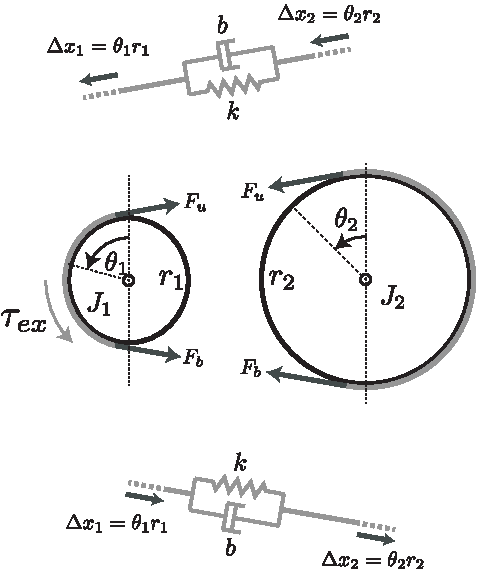
\includegraphics[width=0.9\textwidth]{beltpulleyelastic_sol}
    \end{center}
\end{minipage}

\vspace{12pt}

Let's first write the spring force relations
%
\begin{align*}
  F_u &= k \left( \Delta x_1 - \Delta x_2 \right) + b \frac{d}{d t}
        \left( \Delta x_1 - \Delta x_2 \right)
  \\
    &= k \left(r_1 \theta_1 -r_2 \theta_2 \right) + b  \left( r_1
      \dot{\theta}_1 - r_2 \dot{\theta}_2 \right)
\\
    &= k r_1 \theta_1 - k r_2 \theta_2 + b r_1 \dot{\theta}_1 - b r_2
      \dot{\theta}_2
\\
  F_b &= k \left( -\Delta x_1 + \Delta x_2 \right) + b \frac{d}{d t}
        \left( -\Delta x_1 + \Delta x_2 \right)
  \\
    &= k \left(-r_1 \theta_1 + r_2 \theta_2 \right) + b  \left( -r_1
      \dot{\theta}_1 + r_2 \dot{\theta}_2 \right)
\\
    &= -k r_1 \theta_1 + k r_2 \theta_2 - b r_1 \dot{\theta}_1 + b r_2
      \dot{\theta}_2
\end{align*}

Now let's write the equations of motion of the individual bodies
%
\begin{align*}
  J_1 \ddot{\theta_1} &= \tau_{ex} - F_u r_1 + F_b r_1
  \\
  &= \tau_{ex} + \left(  -k r_1^2 \theta_1 + k r_2 r_1 \theta_2 - b
    r_1^2 \dot{\theta}_1 + b r_2 r_1
      \dot{\theta}_2 \right) + \left( -k r_1^2 \theta_1 + k r_2 r_1
    \theta_2 - b r_1^2 \dot{\theta}_1 + b r_2 r_1
      \dot{\theta}_2 \right)
\\
&= \tau_{ex} - 2 k r_1^2 \theta_1 +2 k r_2 r_1 \theta_2 - 2 b
    r_1^2 \dot{\theta}_1 + 2 b r_2 r_1 \dot{\theta}_2 
\\
 J_2 \ddot{\theta_2} &= F_u r_2 - F_b r_2
\\
  &= \left( k r_1 r_2 \theta_1 - k r_2^2 \theta_2 + b r_1 r_2 \dot{\theta}_1 - b r_2^2
      \dot{\theta}_2 \right) + \left( k r_1 r_2 \theta_1 - k r_2^2 \theta_2 + b r_1 r_2 \dot{\theta}_1 - b r_2^2
      \dot{\theta}_2 \right) 
\\
&= 2 k r_1 r_2 \theta_1 - 2 k r_2^2 \theta_2 + 2 b r_1 r_2
  \dot{\theta}_1 - 2 b r_2^2 \dot{\theta}_2
\end{align*}

\begin{enumerate}
	\item Let $\mathbf{x} = \left[ \theta_1 \ \dot{\theta}_1 \
            \theta_2 \ \dot{\theta}_2 \right]^T$, then we can find a
          state-space representation
%
\begin{align*}
\dot{\mathbf{x}} &= \left[ \begin{array}{cccc} 0 & 1 & 0 & 0 \\
-\frac{2 k r_1^2}{J_1} & -\frac{2 b r_1^2}{J_1} & \frac{2 k r_1 r_2}{J_1} &
\frac{2 b r_1 r_2}{J_1}
\\
0 & 0 & 0 & 1 \\
\frac{2 k r_1 r_2}{J_2} & \frac{2 b r_1 r_2}{J_2} & -\frac{2 k r_2^2}{J_2} &
-\frac{2 b r_2^2}{J_2}
\end{array} \right] \mathbf{x} +
                   \left[ \begin{array}{c} 0 \\ \frac{1}{J_1} \\ 0 \\
                            0 \end{array} \right] u
\\
y &= \left[ \begin{array}{cccc} 0 & 0 & 1 & 0 \end{array} \right] \mathbf{x} 
\end{align*}

	\item Let's take the Laplace transform of the derived
          diffferential equations

\begin{align*}
\left[  J_1 s^2 + 2 b r_1^2 s + 2 k r_1^2 \right] \Theta_1(s) &= U(s)
                                                                +
\left[ 2 b r_2 r_1 s + 2 k r_2 r_1 \right] Y(s)
\\
\left[  J_2 s^2 + 2 b r_2^2 s + 2 k r_2^2 \right] Y(s) &= 
\left[ 2 k r_1 r_2 + 2 b r_1 r_2 s \right] \Theta_1(s)
\end{align*}

In order to simplify the expression let
%
\begin{align*}
B_1 = 2 b r_1^2 \ , \ K_1 = 2 k r_1^2 \ , \ B_2 =2 b r_2^2 \ , \ K_2 =
  2 k r_2^2 \ , \ B_{12} = 2 b r_2 r_1 \ , \ K_{12} = 2 k r_1 r_2
\end{align*}
%
Then we can have 
%
\begin{align*}
&\left[  J_1 s^2 + B_1 s + K_1 \right] \Theta_1(s) = U(s)
                                                                +
\left[ B_{12} s + K_{12} \right] Y(s)
\\
&\left[  J_2 s^2 +B_2 s+ K_2 \right] Y(s) = 
\left[ B_{12} s +  K_{12} \right] \Theta_1(s) \quad \rightarrow \quad 
\Theta_1(s) = \frac{\left[  J_2 s^2 +B_2 s+ K_2 \right]}{\left[
                                           B_{12} s + K_{12}
                                           \right]} Y(s)
\\
&Y(s) \left\lbrace \left[  J_1 s^2 + B_1 s + K_1 \right] \frac{\left[
  J_2 s^2 +B_2 s+ K_2 \right]}{\left[ B_{12} s + K_{12}\right]} -
  \left[ B_{12} s + K_{12} \right]\right\rbrace = U(s)
\\
&Y(s) \left\lbrace \left[  J_1 s^2 + B_1 s + K_1 \right] \frac{\left[
  J_2 s^2 +B_2 s+ K_2 \right]}{\left[ B_{12} s + K_{12}\right]} -
  \left[ B_{12} s + K_{12} \right]\right\rbrace = U(s)
\end{align*}

Let $\frac{Y(s)}{U(s)} = \frac{N(s)}{D(s)}$, then

\begin{align*}
D(s) =& J_1 J_2 s^4 + (B_1 J_2 + B_2 J_1) s^3 + (- B_{12}^2 + B_1 B_2 + J_1 K_2 +
  J_2 K_1) s^2 
\\&+ (B_1 K_2 + B_2 K_1 - 2 B_{12} K_{12}) s + ( -
  K_{12}^2 + K_1 K_2 )
\\
D(s) =&  J_1 J_2 s^4 + (B_1 J_2 + B_2 J_1) s^3 + ( J_1 K_2 + J_2 K_1)
        s^2 + 0 + 0
\end{align*}

Finally the transfer function can be computed as

\begin{align*}
\frac{Y(s)}{U(s)} = \frac{ B_{12} s + K_{12} }{ J_1 J_2 s^4 + (B_1 J_2 + B_2 J_1) s^3 + ( J_1 K_2 + J_2 K_1)
        s^2 }
\end{align*}

\item The state-space representation with the given coefficients take the form
%
 \begin{align*}
\dot{\mathbf{x}} &= \left[ \begin{array}{cccc} 0 & 100 & 0 & 0 \\
-50 & -5 & 100 & 10
\\
0 & 0 & 0 & 1 \\
10 & 1 & -20 & -2
\end{array} \right] \mathbf{x} +
                   \left[ \begin{array}{c} 0 \\ 1 \\ 0 \\
                            0 \end{array} \right] u
\\
y &= \left[ \begin{array}{cccc} 0 & 0 & 1 & 0 \end{array} \right] \mathbf{x} 
\end{align*}

Transfer function with the given coefficients take the form
%
 \begin{align*}
 G(s) = \frac{Y(s)}{U(s)} = \frac{100 (s + 10)}{s^4 + 7 s^3 + 70 s^2}
 \end{align*}
 %
 
A sample MATLAB code piece which converts the state-space form to the transfer function form
(in terms of numerator and denumerator coefficients) is provided below. It is clear that, the computed
coefficients match the previous ones. 
 
     \vspace{12pt}
    
\begin{minipage}[h]{1\linewidth}
    \begin{center}
      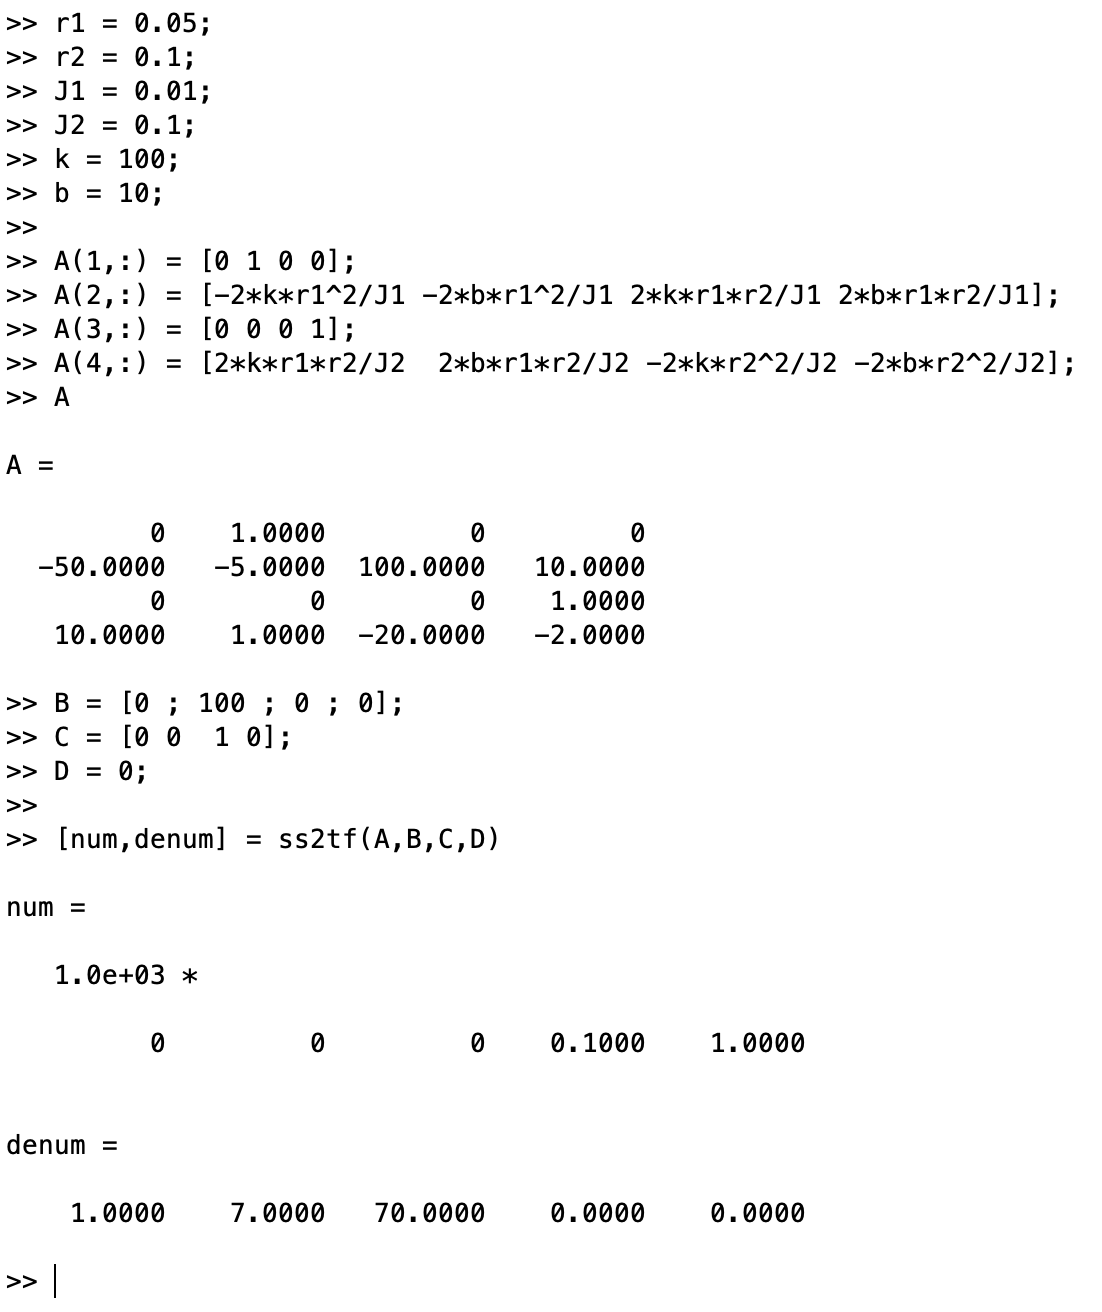
\includegraphics[width=0.75\textwidth]{matlabver}
    \end{center}
\end{minipage}

\end{enumerate}

%%%%%%%%%%%%%%%%%%%%%%%

\newpage

\begin{exmp}
Mehcanical system with ideal lever
\end{exmp}
 
 \vspace{-30pt}
  
\begin{minipage}[h]{1\linewidth}
    \begin{center}
      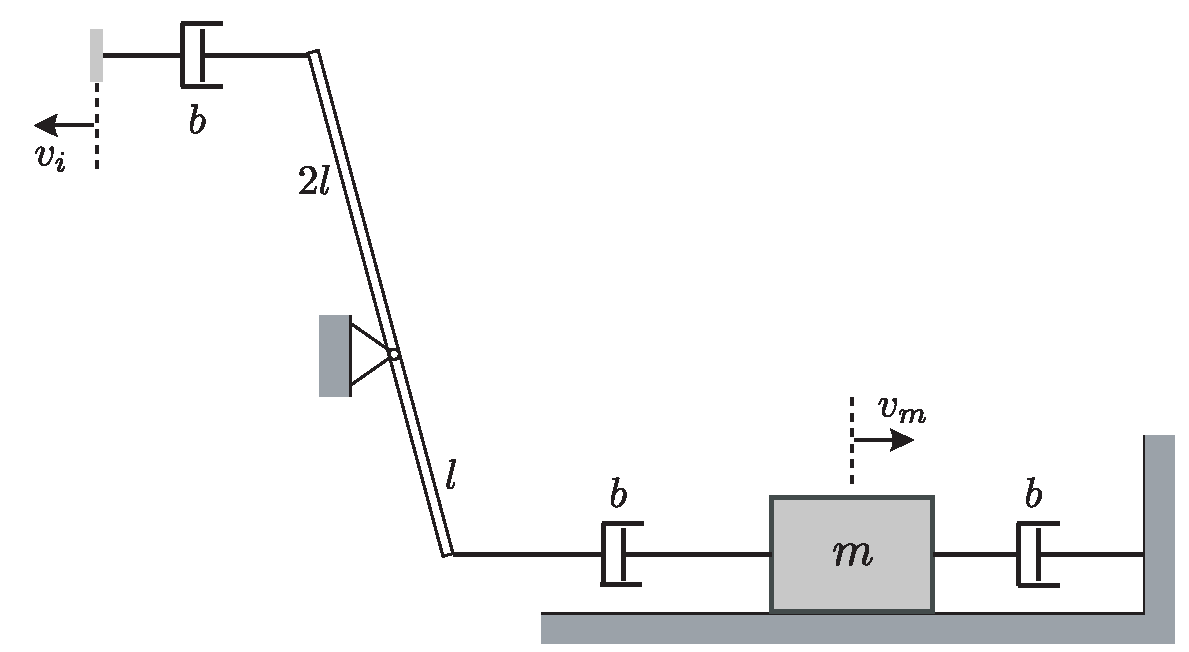
\includegraphics[width=0.6\textwidth]{leverideal}
    \end{center}
\end{minipage}   

\vspace{6pt}

Input--output of the system is the are $u(t) = v_i(t)$, and
$y(t) = v_m(t)$ respectively. If we draw the free body diagram of
the mass and draw the kinematic realtions of the lever we 
obtain the following illsutration

\vspace{6pt}
  
\begin{minipage}[h]{1\linewidth}
    \begin{center}
      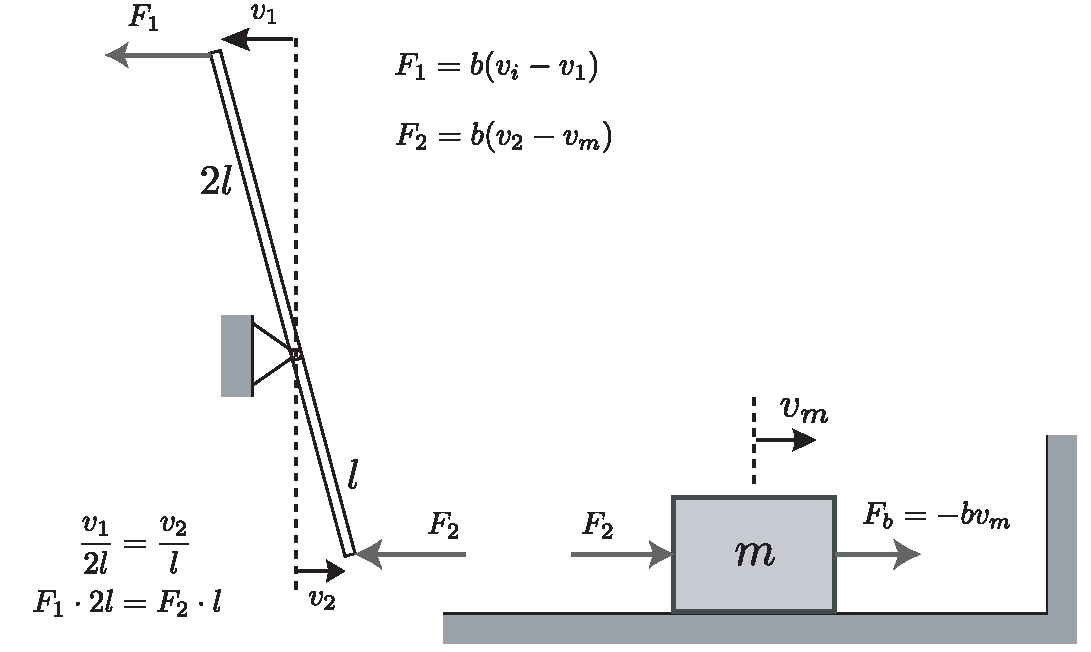
\includegraphics[width=0.75\textwidth]{leverideal_solution}
    \end{center}
\end{minipage}   

\vspace{6pt}

First let's concentrate on the lever side and try to eliminate
intermediate variables
%
\begin{align*}
  2 F_1 &= F_2  \\
  2 (v_i - v_1)  &= (v_2 - v_m) \\
  v_2 + 2 v_1 &= 2 v_i + v_m  \\
  v_2 &= \frac{2}{5} v_i + \frac{1}{5} v_m            
\end{align*}
%
Now let's write equations of motion for the single body
%
\begin{align*}
  m \dot{v}_M &= F_2 + F_b \\
  m \dot{v}_M &= b ( v_2 - v_m ) - b v_m \\
  \dot{v}_M &=  \frac{2}{5} v_i + \frac{1}{5} v_m  - v_m - v_m \\
  \dot{v}_M + \frac{9}{5} v_m &=  \frac{2}{5} v_i \\
   \dot{y} + \frac{9}{5} y &=  \frac{2}{5} u
\end{align*}
%
Transfer function simply takes the form
%
\begin{align*}
  \frac{Y(s)}{U(s)} = \frac{2/5}{s + 9/5}
\end{align*}
%
%%%%%%%%%%%%%%%%%%%%%%%

\begin{exmp}
Mehcanical system with an non-ideal lever that has an inertia of $J = m l^2$
\end{exmp}

\vspace{6pt}
  
\begin{minipage}[h]{1\linewidth}
    \begin{center}
      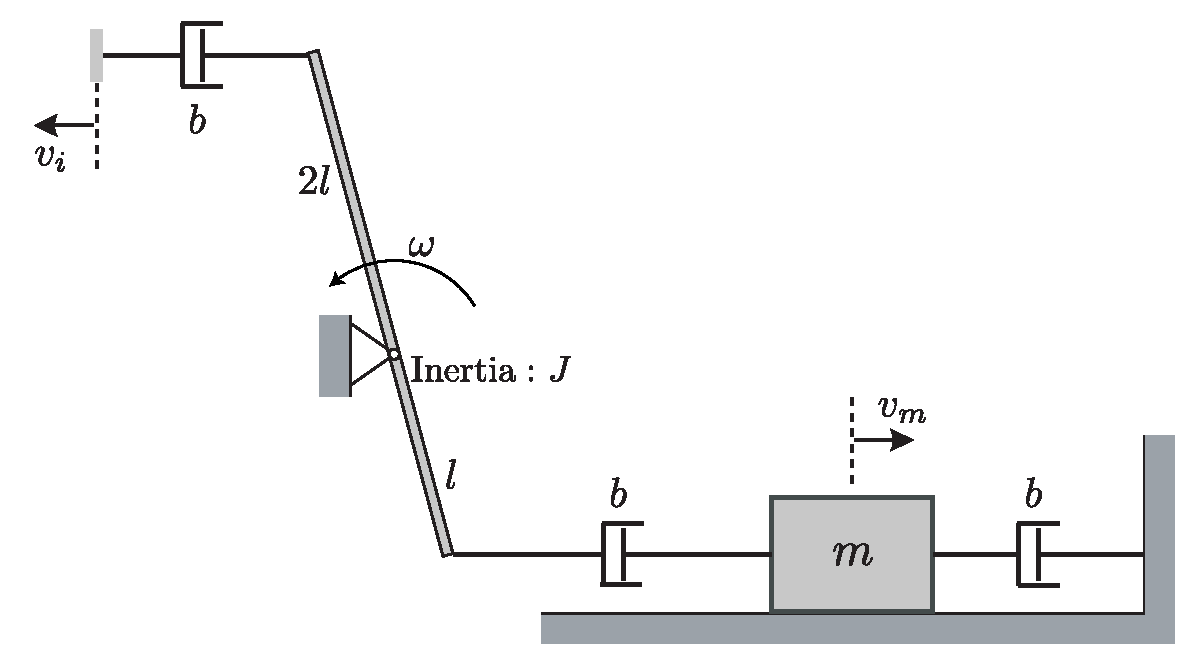
\includegraphics[width=0.6\textwidth]{lever}
    \end{center}
\end{minipage}   

\vspace{6pt}

Input--output of the system is the are $u(t) = v_i(t)$, and
$y(t) = v_m(t)$ respectively. If we draw the free body diagrams of
the lever and the mass, and derive the force relations we obtain

\vspace{12pt}
  
\begin{minipage}[h]{1\linewidth}
    \begin{center}
      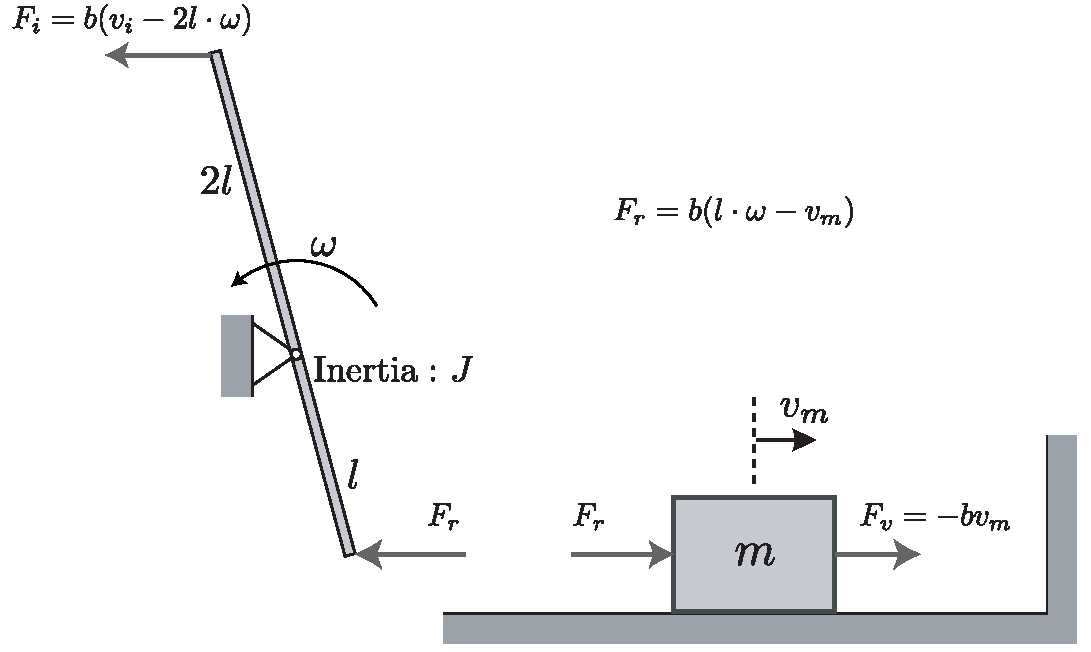
\includegraphics[width=0.75\textwidth]{lever_solution}
    \end{center}
\end{minipage}   

\vspace{12pt}

If we write equations of motion for the lever and the mass, 
we obtain following differnetial equations
%
\begin{align*}
  J \dot{\omega} &= F_i \times 2l - F_r \times l  = (- 5 l^2 b) \omega + (2 l b) v_i + (l b) v_m 
  \\
\dot{\omega} + \frac{5 b}{m} \omega &= \frac{b}{m l} v_m + \frac{2
                                          b}{m l} v_i
  \\
\dot{\omega} + 5 \omega &= \frac{1}{l} v_m + \frac{2}{l} v_i
\\
,
\\
m \dot{v}_m &= F_r + F_v  = (- 2 b) v_m + ( b l ) \omega
\\
 \dot{v}_M + \frac{2 b}{m} v_m  &= \frac{ b l }{m} \omega
\\
 \dot{v}_M + 2 v_m  &= l \, \omega
\end{align*}

If we take the Laplace transform of the derived differential equations
%
\begin{align*}
\Omega(s) \left[ s + 5 \right] &= \frac{1}{l} Y(s) + \frac{2}{l} U(s)
\\
Y(s) \left[ s + 2 \right] &= l \, \Omega(s)
\\
Y(s) \left[ s + 2 \right]\left[ s + 5 \right] \frac{1}{l} &=
                                                            \frac{1}{l}
                                                            Y(s) +
                                                            \frac{2}{l}
                                                           2 U(s)
\\
Y(s) ( s + 2 ) ( s + 5 ) &= Y(s) + 2 U(s)
\\
\frac{Y(s)}{U(s)} &= \frac{2}{s^2 + 7 s + 11}
\end{align*}

\vspace{12pt}

Now let's find a state-space representation for the given system. The
ODE representation of the transfer function has the following form
%
\begin{align*}
  \ddot{y} + 7 \dot{y} + 11 y = 2 u
\end{align*}
%
The system is a $2^{nd}$ order dynamical system. Let $\mathbf{x} = [y
\ \dot{y}]^T$, then 
%
\begin{align*}
  \dot{x_1} &= \dot{y} = x_2 \\
  \dot{x_2} &= \ddot{y} = -7 \dot{y} - 11 y + 2 u  
              = -7 x_2 - 11 x_1 +2 u  \\
  y &= x_1
\end{align*}
%
The state-representation with the chosedn state definition takes the form
 \begin{align*}
\dot{\mathbf{x}} &= \left[ \begin{array}{cc} 0 & 1\\
-11 & -7 
\end{array} \right] \mathbf{x} +
\left[ \begin{array}{c} 0 \\ 1 \end{array} \right] u
\\
y &= \left[ \begin{array}{cccc} 1 & 0 \end{array} \right] \mathbf{x} 
+ [ 0 ] u
\end{align*}

% **** This ENDS THE EXAMPLES. DON'T DELETE THE FOLLOWING LINE:
\end{document}